\documentclass{scrbook}
\usepackage{graphicx} % Required for inserting images
\usepackage{tabularx} % Required for fixed width tables
\usepackage{scrlayer-scrpage} % Required for the subtitles
\usepackage{url} % Required for the URLs
\usepackage{hyperref} % Required for the URLs
\usepackage{listings} % Required for the code snippets
\usepackage{mathtools} % Required for the system of equations
\usepackage{amsmath,amssymb} % Required for some math symbols
\usepackage{enumitem} % Required for lettered lists

% Put the caption of the snippets at the bottom
\lstset{
    captionpos=b
}


\title{Solidity}
\subtitle{Ambient intelligence course (A.Y. 2025/2026)\\Topic taught by Prof. Arnaldo Tomasino}
\author{Gabriele Colapinto}
\date{\today}

\begin{document}

\maketitle
\thispagestyle{empty}

{\Large\textbf{License}} \\
{Notes from Ambient intelligence (A.Y. 2025/2026) by Gabriele Colapinto. 
Course taught by professors Michele Ruta, Floriano Scioscia, Arnaldo Tomasino, Davide Loconte — 
Licensed under CC BY-NC 4.0.\\
\url{https://creativecommons.org/licenses/by-nc/4.0/}}

\vspace*{\fill}
\rule{\textwidth}{0.2pt}
\small{© 2025 Gabriele Colapinto \\
Released under the \href{https://creativecommons.org/licenses/by-nc/4.0/}{Creative Commons Attribution–NonCommercial 4.0 International License}}

\clearpage

\tableofcontents

\chapter{Introduction to High-Level Languages for the Ethereum Virtual Machine (EVM)}

The Ethereum Virtual Machine (EVM) is the runtime environment for smart contracts in Ethereum. While the EVM executes low-level instructions known as bytecode, developers write smart contracts using more abstract, human-readable high-level languages. These languages provide structures, data types, and syntax that are more intuitive and manageable than raw bytecode, which they ultimately compile down to for execution on the blockchain. This abstraction is crucial for building complex and secure decentralized applications.\\

\textbf{Solidity} stands as the primary language in this domain. It is an object-oriented, high-level language designed specifically for implementing smart contracts that govern the behavior of accounts within the Ethereum state. Its key characteristics include being a curly-bracket language, heavily influenced by C++, Python, and JavaScript, making it familiar to a broad range of developers. Furthermore, Solidity is statically typed, meaning the type of every variable must be declared at compile time, which enhances code clarity and helps prevent common errors.\\

While Solidity is the most prominent, other languages have also been developed for the EVM. The table below provides a comparison of the key options.

\begin{table}[h!]
    \centering
    \begin{tabular}{|p{0.2\textwidth}|p{0.35\textwidth}|p{0.35\textwidth}|}
        \hline
        Language & Key Characteristics & Status \\ \hline
        
        \textbf{Solidity} & Object-oriented, statically typed, and specifically designed for the EVM. Influenced by C++, Python, and JavaScript. & The most mature, widely supported, and actively developed language for Ethereum and other EVM-compatible blockchains. \\ \hline
        
        \textbf{Serpent} & A Python-like language that was one of the early options for Ethereum development. & Deprecated due to security vulnerabilities. No longer recommended for use. \\ \hline
        
        \textbf{Vyper} & A newer, Python-like, object-oriented language that serves as a viable alternative to Solidity. & Actively developed and serves as a viable alternative to Solidity. \\ \hline
    \end{tabular}
\end{table}

Ultimately, Solidity's maturity, extensive documentation, large developer community, and broad toolchain support have solidified its position as the de facto standard for smart contract development. It has been adopted not only by Ethereum but by numerous other blockchain platforms that use EVM-compatible virtual machines. For both security and functionality, it is a critical best practice to use the latest released version of the Solidity compiler for any new project, ensuring access to the most recent features and security fixes.

\chapter{The Solidity Development Environment}

Before writing the first line of code, a developer must select a suitable development environment and toolset. The Solidity ecosystem offers a variety of options to accommodate different workflows and preferences, from simple browser-based Integrated Development Environments (IDEs) for quick prototyping to sophisticated command-line compilers for integration into complex development pipelines.\\

The primary options for working with Solidity are:

\begin{enumerate}
    \item \textbf{Remix IDE:} An open-source, browser-based IDE that provides a complete environment for writing, compiling, deploying, and debugging Solidity smart contracts. It is ideal for rapid prototyping and educational purposes due to its immediate accessibility without any local installation.
    
    \item \textbf{The} \texttt{\textbf{solc}} \textbf{Solidity Compiler:} This is the foundational command-line compiler for Solidity, written in C++. Developers can install it on their local machines through pre-compiled binary packages or by building it directly from the source code.
    
    \item \textbf{Docker Images:} For developers who prefer containerized environments, official Docker images containing the \texttt{solc} compiler are available. This approach simplifies dependency management and ensures a consistent build environment. A combination of \texttt{solc} and Docker is particularly suited for professional, collaborative projects requiring reproducible builds and integration with CI/CD pipelines.
    
    \item \texttt{\textbf{solcjs}} \textbf{(Npm/Node.js):} This is a JavaScript binding for the Solidity compiler, distributed as an npm package. It is a subset of the C++ \texttt{solc} codebase and has a significant trade-off: \texttt{solcjs} has reduced features compared to the full \texttt{solc} compiler. However, its primary advantage is the ability to be used directly within JavaScript and Node.js projects, allowing for programmatic compilation and deployment as part of an integrated workflow.
\end{enumerate}

As Solidity is a language in constant evolution, with new features and bug fixes introduced regularly, it is a crucial best practice to use the latest released version for new projects. This ensures that contracts are compiled with the most up-to-date security checks and language features.

\chapter{Anatomy of a Solidity Source File}

Every Solidity source file, identified by the \texttt{.sol} extension, follows a conventional structure that is fundamental to writing clear, secure, and compiler-compatible code. This structure is not merely a stylistic convention but a set of directives and declarations that inform the compiler about licensing, language version, dependencies, and the core logic of the smart contracts within. A typical source file includes license identifiers, version pragmas, import statements, and one or more contract definitions.

\begin{lstlisting}[caption={Simple contract with one function that returns the "Hello, World!" string when called}]
    pragma solidity ^0.6.0;
    contract HelloWorld {
        function helloWorld() external pure returns (string memory) {
            return "Hello, World!";
        }
    }
\end{lstlisting}

\section{SPDX License Identifier}

To foster trust and transparency in the open-source ecosystem of smart contracts, the Solidity compiler encourages the use of machine-readable SPDX (Software Data Package Exchange) license identifiers. Every source file should begin with a comment specifying the software license under which the code is made available.

\begin{lstlisting}
    // SPDX-License-Identifier: MIT
\end{lstlisting}

This comment, which is recommended at the top of the file, does not represent a legal validation by the compiler. Instead, the compiler includes the provided string in the contract's bytecode metadata, making the license programmatically verifiable. For proprietary or closed-source code where no license is specified, the special value \texttt{UNLICENSED} should be used.

\section{Pragmas}

The \texttt{pragma} keyword serves as a directive to the compiler, enabling specific features or enforcing certain checks. Pragma directives are always local to the source file in which they are declared; they are not inherited by other files, even when one file imports another. This ensures that each file's compilation settings are explicit and self-contained.

\begin{itemize}
    \item \textbf{Version Pragma:} This is the most critical pragma. Its purpose is to instruct the compiler to check its own version against the version(s) specified in the source file, rejecting compilation if there is an incompatibility. This prevents unintended behavior that can arise from using a contract with a compiler version for which it was not designed. Solidity follows a \texttt{major.minor.bugfix} versioning scheme.
    \begin{itemize}
        \item \texttt{pragma solidity \textasciicircum0.5.2;} allows compilation by any compiler version from \texttt{0.5.2} up to, but not including, \texttt{0.6.0}. The caret \texttt{\textasciicircum} is a convenient way to allow non-breaking bugfix releases while protecting against potentially breaking changes in the next minor version.
        
        \item \texttt{pragma solidity >=0.5.2 <0.7.0;} provides a more explicit range, accepting any version from \texttt{0.5.2} up to, but not including, \texttt{0.7.0}. It is important to note that this pragma \textit{instructs the compiler to check its version}; it does not change the compiler's version or enable/disable features.
    \end{itemize}
    
    \item \textbf{ABI Coder Pragma} (e.g.: \texttt{pragma abicoder v2;}) \textbf{:} This pragma selects the implementation of the Application Binary Interface (ABI) encoder and decoder. The \texttt{v2} coder, which is the default from Solidity 0.8.0, is more powerful and secure than the legacy \texttt{v1} coder. It supports complex data types like nested arrays and structs in function arguments and return values and performs more extensive validation.
    
    \item \textbf{Experimental Pragma:} This pragma is used to enable features that are still under development and not enabled by default. For example \texttt{pragma experimental ABIEncoderV2;} was used to select the second version of the ABI encoder when it was still experimental and \texttt{pragma experimental SMTChecker} is used to enable advanced static analysis.
\end{itemize}

\section{Importing Other Source Files}

Solidity supports \texttt{import} statements to facilitate code modularization, allowing developers to organize their projects into reusable components. To ensure reproducible builds, the compiler manages source files in a \textbf{virtual filesystem (VFS)}. This means import paths do not refer directly to the host filesystem but to unique source unit names within this VFS, abstracting away system-specific details.\\

Several import syntaxes are available:

\begin{itemize}
    \item \texttt{import "filename";}: Imports all global symbols from the specified file into the current global scope. This form is not recommended because it unpredictably pollutes the namespace; any new global symbols added to the imported file will automatically appear in the current file's scope, potentially causing naming conflicts.
    
    \item \texttt{import * as symbolName from "filename";}: Creates a new global symbol (\texttt{symbolName}) that acts as a namespace for all global symbols from the imported file. If we use this syntax we can access the imported symbols as follows: \texttt{symbolName.symbol}.
    
    \item \texttt{import "filename" as symbolName;}: An alternative syntax that is equivalent to the one above.
\end{itemize}

\section{Comments and NatSpec}

Solidity supports standard single-line (\texttt{//}) and multi-line (\texttt{/*...*/}) comments. Additionally, it defines a special format for documentation known as the \textbf{Ethereum Natural Language Specification Format (NatSpec)}. NatSpec comments are written with a triple slash (\texttt{///}) or a double-asterisk block (\texttt{/** ... */}) and are placed directly above contract, function, and state variable declarations.\\

NatSpec provides a standardized way to create rich documentation for a contract's public interface. It uses Doxygen-inspired tags to describe different aspects of the code:

\begin{itemize}
    \item \texttt{@title}: A title for the contract or interface.
    
    \item \texttt{@author}: The name of the author.
    
    \item \texttt{@notice}: A user-facing explanation of what the contract or function does. This is intended for end-users interacting with the contract.
    
    \item \texttt{@dev}: A developer-facing explanation with extra details or technical considerations.
    
    \item \texttt{@param}: Documents a function's parameter, followed by the parameter name and a description.
    
    \item \texttt{@return}: Documents a function's return variable(s).
\end{itemize}

\begin{lstlisting}[caption={Example of function with comments}]
    pragma solidity >=0.4.0 <0.7.0;
    
    /** @title Shape calculator. */
    contract ShapeCalculator {
        /// @dev Calculates a rectangle's surface and perimeter.
        /// @param w Width of the rectangle.
        /// @param h Height of the rectangle.
        /// @return s The calculated surface.
        /// @return p The calculated perimeter.
        function rectangle(uint w, uint h) public pure returns (uint s, uint p) {
            s = w * h;
            p = 2 * (w + h);
        }
    }
\end{lstlisting}

The Solidity compiler can parse these NatSpec comments and generate a machine-readable JSON output, which can be used by developer tools and user interfaces to provide contextual information to both developers and end-users.\\

Together, these structural elements—license identifiers, pragmas, imports, and documentation—form the foundation for writing professional, maintainable, and secure Solidity code, setting the stage for defining the core logic within contracts.

\chapter{Data Types in Solidity}

Solidity is a statically typed language, which means that the data type of every variable must be explicitly declared at compile time. This strictness helps prevent a wide range of bugs by ensuring that operations are only performed on compatible types. Data types in Solidity are broadly categorized into two groups: \textbf{Value Types} and \textbf{Reference Types}. The fundamental difference between them lies in how they are stored and passed around in the code: value types are always passed by value (a full copy is made), while reference types are passed by reference (a pointer to the data's location is passed).

\section{Value Types}

Value types are fundamental data types where variables hold their own data directly. When a value type variable is assigned to another variable or passed as an argument to a function, an independent copy of the data is created. Modifying the copy does not affect the original variable.\\

The main value types in Solidity include:

\begin{itemize}
    \item \textbf{Boolean (}\texttt{\textbf{bool}}\textbf{):} A type that can hold one of two possible values: \texttt{true} or \texttt{false}.
    
    \item \textbf{Integer (}\texttt{\textbf{intN}}\textbf{/}\texttt{\textbf{uintN}}\textbf{):} Signed (\texttt{int}) and unsigned (\texttt{uint}) integers of various sizes. \texttt{N} represents the number of bits and can be specified in steps of 8, from 8 to 256 (e.g., \texttt{uint8}, \texttt{int32}, \texttt{uint256}). If the size is not specified, \texttt{int} and \texttt{uint} are aliases for \texttt{int256} and \texttt{uint256}, respectively.
    
    \item \textbf{Bytes (}\texttt{\textbf{bytesN}}\textbf{):} A fixed-size sequence of bytes. The size \texttt{N} can range from 1 to 32 (e.g., \texttt{bytes1}, \texttt{bytes32}). The keyword \texttt{byte} is an alias for \texttt{bytes1}.
    
    \item \textbf{Address:} A 20-byte value type specifically designed to hold an Ethereum account address. It has several built-in members accessible with dot notation, such as \texttt{.balance} which returns the account's balance in wei. Hexadecimal literals that are 40 hex digits long and pass a checksum test are treated as addresses.
    \begin{itemize}
        \item There is a special variant, \texttt{\textbf{address payable}}, which is an address that can receive Ether. This type has additional members: \texttt{transfer} and \texttt{send}, which are functions for sending Ether to the address. A standard \texttt{address} cannot receive Ether directly via these methods.
        The function \texttt{transfer(uint256 amount)} forwards 2300 gas by default and is reverted upon failure while the function \texttt{send(uint256 amount)} does not revert upon failure but returns \texttt{false} instead.
    \end{itemize}
\end{itemize}

\section{Reference Types}

Reference types, in contrast to value types, do not store data directly within the variable. Instead, they store a reference (or pointer) to the location where the data resides. This has a critical implication: assigning a reference variable to another or passing it to a function creates a new reference to the \textit{same} underlying data. Therefore, modifying the data through one reference variable will be visible to all other variables that refer to that same data location.\\

For reference types, it is mandatory to explicitly specify the \textbf{Data Location} where the variable's data is stored. There are three possible data locations:

\begin{itemize}
    \item \texttt{memory}: This location is temporary and is used to hold data during the execution of an external function call. Its lifecycle is tied to the function call; once the function completes, the memory is cleared. It is a less expensive, temporary alternative to \texttt{storage}.
    
    \item \texttt{storage}: This is the persistent, on-chain location where a contract's state variables are stored. Data in storage survives across transactions and is the primary component of a contract's state. It is the most gas-expensive location due to its persistence on the blockchain.
    
    \item \texttt{calldata}: A special, read-only data location that contains the arguments passed to an external function. It is immutable and is the most gas-efficient location for function arguments because it is read-only and requires no copying to memory.
\end{itemize}

\begin{lstlisting}[caption={Reference variable declaration syntax}]
    _Type _DataLocation _VariableName
\end{lstlisting}

An assignment that moves data from one location to another (e.g., from \texttt{storage} to \texttt{memory}) always incurs a copy operation while assignments inside the same data location only copy in some cases.

\subsection{Arrays}

Arrays are collections of elements of the same type. Solidity supports two kinds of arrays:

\begin{itemize}
    \item \textbf{Fixed-size arrays:} Declared with a compile-time constant size, e.g., \texttt{uint[8]}.
    
    \item \textbf{Dynamic-size arrays:} Declared without a fixed size, e.g., \texttt{uint[]}. It's important to note that while dynamic arrays in \texttt{storage} can grow freely, dynamic arrays in \texttt{memory} must be created with a specified maximum size at the time of declaration (e.g., \texttt{new uint[](size)}), allocating a fixed block of memory.
\end{itemize}

Arrays have several built-in members, including \texttt{.length} to get the number of elements. For dynamic arrays located in \texttt{storage}, \texttt{.push()} can be used to append an element, and \texttt{.pop()} can be used to remove the last element. Array slicing (\texttt{x[start:end]}) is also supported.\\

Two special types are treated as arrays:

\begin{itemize}
    \item \texttt{bytes}: A dynamic-size byte array.
    
    \item \texttt{string}: A dynamic-size UTF-8 encoded string. While functionally similar to a byte array, \texttt{string} variables do not allow access by index or a \texttt{.length} member. Furthermore, Solidity does not have built-in functions for string manipulation, requiring the use of external libraries.
\end{itemize}

\subsection{Mappings}

Mappings are key-value pair data structures, analogous to hash tables. They are declared using the syntax \texttt{mapping(\_KeyType => \_ValueType) \_VariableName}. Mappings have one critical rule: they can \textbf{only} have \texttt{storage} as their data location and are primarily used for state variables.

\begin{lstlisting}[caption={Example of mapping declaration and usage}, label={lbl:mapping}]
    pragma solidity >=0.4.0 <0.7.0;
    
    contract MappingExample {
        mapping(address => uint) public balances;
        
        function update(uint newBalance) public {
            balances[msg.sender] = newBalance;
        }
    }
    
    contract MappingUser {
        function f() public returns (uint) {
            MappingExample m = new MappingExample();
            m.update(100);
            return m.balances(address(this));
        }
    }
\end{lstlisting}

The code in snippet \ref{lbl:mapping} contains two contracts. The first contract declares a mapping as an attribute containing the association between an address and an unsigned integer (of size 256 by default) which is the balance of the address. The second contract contains a function that uses the first contract as an object, updates the balance and then returns it. It's important to notice that specifying the address of the account whose balance will be changed is not necessary because the \texttt{update} function automatically refers to the address of the account sending the updating request (\texttt{msg.sender}).

\subsection{Structs and Enums}

Solidity allows developers to define their own complex types:

\begin{itemize}
    \item \texttt{\textbf{struct}}: A way to create a custom, user-defined type that can group together variables of different types, useful for organizing related data.

    \begin{lstlisting}[caption={struct example}]
        struct StructExample {
            uint[] contents;
            uint moreInfo;
            mapping(uint => StructExample) mappingExample;
        }
    \end{lstlisting}
    
    \item \texttt{\textbf{enum}}: A way to create a user-defined type that represents a finite set of constant values. Internally, enum options are represented as consecutive unsigned integers starting from 0.

    \begin{lstlisting}[caption={enum example}]
        enum ActionChoices { GoLeft, GoRight, GoStraight, SitStill }
    \end{lstlisting}
\end{itemize}

Understanding the distinction between value and reference types, along with the proper use of data locations, is fundamental to writing gas-efficient and secure smart contracts, as it directly impacts how data is stored, manipulated, and paid for on the blockchain.

\chapter{Operators and Control Structures}

Like any mature programming language, Solidity provides a comprehensive set of operators and control structures to implement complex logic within functions. These tools allow developers to perform calculations, make decisions, and control the flow of execution in their smart contracts.

\section{Operators}

Solidity's operators are largely familiar to developers with a background in C or JavaScript. They are grouped here by the data types they apply to:

\begin{itemize}
    \item \textbf{Boolean:}
    \begin{itemize}
        \item Logical operators: \texttt{!} (not), \texttt{\&\&} (and), \texttt{||} (or)
        \item Comparison operators: \texttt{==} (equality), \texttt{!=} (inequality)
    \end{itemize}
    
    \item \textbf{Integer:}
    \begin{itemize}
        \item Comparison operators: \texttt{<=}, \texttt{<}, \texttt{==}, \texttt{!=}, \texttt{>=}, \texttt{>} (all evaluate to a \texttt{bool})
        \item Bitwise operators: \texttt{\&} (and), \texttt{|} (or), \texttt{\textasciicircum} (xor), \texttt{\textasciitilde} (negation)
        \item Shift operators: \texttt{<<} (left shift), \texttt{>>} (right shift)
        \item Arithmetic operators: \texttt{+}, \texttt{-}, \texttt{*}, \texttt{/}, \texttt{\%} (modulo), \texttt{**} (exponentiation)
    \end{itemize}
    
    \item \textbf{Byte Array:}
    \begin{itemize}
        \item Comparison, bitwise, and shift operators are available.
        \item Index access \texttt{x[k]} allows reading the \textit{k}-th byte (read-only).
    \end{itemize}
    
    \item \textbf{Address:}
    \begin{itemize}
        \item Comparison operators (\texttt{<=}, \texttt{<}, \texttt{==}, \texttt{!=}, \texttt{>=}, \texttt{>}) are available and evaluate to a \texttt{bool}.
    \end{itemize}
\end{itemize}

\section{Control Structures}

Solidity supports standard control flow statements with syntax and semantics that are well-known from other languages.

\begin{itemize}
    \item \texttt{if} / \texttt{if-else} for conditional execution.
    \item \texttt{while} and \texttt{for} for looping.
    \item \texttt{break} and \texttt{continue} to alter loop behavior.
    \item \texttt{return} to exit a function and optionally provide return values.
\end{itemize}

A key difference in Solidity's \texttt{if} statement, stemming from its static and strong typing, is that there is \textbf{no implicit type conversion from non-boolean to boolean types}. For example, code like \texttt{if (1)} which might be valid in C or JavaScript, will cause a compilation error in Solidity. The condition for an \texttt{if} statement must explicitly evaluate to a \texttt{bool}.\\

These foundational elements are the building blocks for constructing the sophisticated business logic and state transitions that define the behavior of a smart contract.

\chapter{Functions and Contracts}

Contracts and functions are the primary architectural components of any Solidity application. A \textbf{contract} is the fundamental building block, serving as a container for state data and the functions that can modify that data. In object-oriented programming terms, a contract is analogous to a class, encapsulating both data (state variables) and behavior (functions) at a specific address on the blockchain.

\section{Functions In-Depth}

Functions define the executable units of code within a contract. They are declared with the \texttt{function} keyword, followed by a name, a list of typed parameters, visibility and state mutability modifiers, and an optional \texttt{returns} clause.

\begin{lstlisting}
    function fname(type1 param1, type2 param2, ..., typeN paramN)
    [modifiers]
    [returns (type1 [res1], type2 [res2], ..., typeN [resN])]
    {
        ...
    }
\end{lstlisting}

Two important state mutability modifiers are \texttt{view} and \texttt{pure}:

\begin{itemize}
    \item \texttt{view} functions promise not to modify the state of the contract. They are permitted to read state variables.
    \item \texttt{pure} functions are even more restrictive; they promise not to read from or modify the state.
\end{itemize}

In Solidity it is possible to overload and override functions.\\

Function calls in Solidity can be either \textbf{Internal} or \textbf{External}:

\begin{itemize}
    \item \textbf{Internal calls} are calls to functions within the same contract instance. These are highly efficient as they are translated by the EVM into a simple \texttt{jump} instruction within the contract's bytecode. Crucially, the memory area is not cleared between internal calls within the same main function execution, allowing memory references to be passed very efficiently. The entire memory space is cleared only after the top-level external call completes.
    
    \item \textbf{External calls} are executed via a message call to another contract's address (or to the same contract, but through its public interface). This process is more gas-intensive as it involves creating and sending a message on the EVM.
\end{itemize}

This efficiency difference makes it a key gas-optimization strategy to design contracts with internal helper functions for complex logic, exposing only a minimal, secure set of functions externally.\\

Function parameters can be passed in two ways:

\begin{enumerate}
    \item \textbf{By Position:} The standard method, where arguments are provided in the same order as the parameters in the function definition.
    
    \item \textbf{By Name:} Arguments can be passed in any order using a \texttt{\{key: value\}} syntax, similar to keyword arguments in Python. For example: \texttt{set(\{value: 2, key: 3\});}.
\end{enumerate}

\section{The Contract Lifecycle}

A contract, much like a class, can contain declarations for state variables (see snippet ~\ref{lbl:state_variable}), structs, enums, functions, and events. Solidity supports both single and multiple inheritance using the \texttt{is} keyword, allowing contracts to build upon the functionality of others (see snippet ~\ref{lbl:inheritance}).

\begin{lstlisting}[caption={Example of contract with a declaration of a state variable - State variables are permanently stored in contract storage.}, label={lbl:state_variable}]
    pragma solidity >=0.4.0 <0.7.0;
    
    contract SimpleStorage {
        uint storedData; // State variable
        // ...
    }
\end{lstlisting}

\begin{lstlisting}[caption={Inheritance example}, label={lbl:inheritance}]
    contract X { }
    contract Y { }
    contract Z is X, Y { }
\end{lstlisting}

An \texttt{\textbf{abstract}} \textbf{contract} is a contract that cannot be instantiated directly. A contract is considered abstract if at least one of its functions is not implemented, or if it is explicitly marked with the \texttt{abstract} keyword.\\

The \textbf{Constructor} is a special, optional function that is executed only \textbf{once}, when the contract is first created and deployed. A contract can have at most one constructor, declared with the \texttt{constructor} keyword. Its primary use is for initialization logic. The constructor's code is not part of the final bytecode stored on the blockchain.\\

Contracts can also be created from within other contracts using the \texttt{new} keyword. This allows for factory patterns where one contract is responsible for deploying and managing instances of other contracts but with one crucial limitation: the source code (and the
binary) of the created contract has to be known to the creator to avoid cyclic creation dependencies.

\subsection{Cyclic creation}

The cyclic creation is a situation in which two or more contracts try to create each other thus forming a loop. To illustrate why this is impossible let us say that we have contract \texttt{A} and contract \texttt{B} and they try to create each other.

\begin{lstlisting}[caption={Example of direct loop: A $\to$ B $\to$ A}]
    // Contract A
    contract ContractA {
        function createB() public {
            new ContractB();  // A creates B
        }
    }
    
    // Contract B
    contract ContractB {
        function createA() public {
            new ContractA();  // B would like to create A but this is impossible!
        }
    }
\end{lstlisting}

\texttt{A} tries to create \texttt{B} therefore it needs the binary code of the latter. At the same time \texttt{B} tries to create \texttt{A} but this creates a deadlock because no contract can be fully created before the other! \\

Now, let us say that we create a third contract \texttt{C} and we have the following situation:

\begin{lstlisting}[caption={Example of indirect loop: A $\to$ B $\to$ C $\to$ A}]
    contract A {
        function createB() public { new B(); }
    }
    
    contract B {
        function createC() public { new C(); }
    }
    
    contract C {
        function createA() public { new A(); }  // IMPOSSIBLE!
    }
\end{lstlisting}

In this case we have the same problem but through a longer chain.

\subsection{Solution to the cyclic creation}

Let's say that we really want two contracts to refer to each other. We can't use the \texttt{new} keyword because we would incur in the cyclic dependency problem but we can use addresses as follows:

\begin{lstlisting}[caption={Solution to the cyclic dependency problem}]
    contract A {
        address public bAddress;
        
        function setBAddress(address _b) public {
            bAddress = _b;
        }
    }
    
    contract B {
        address public aAddress;
        
        function setAAddress(address _a) public {
            aAddress = _a;
        }
    }
\end{lstlisting}

In this case the contracts are fully deployed separately and linked afterwards so that they refer to each other using addresses instead of code dependency.\\

These concepts—contracts as classes, functions as methods, and a defined lifecycle—provide a robust, object-oriented framework for structuring the logic and state of a decentralized application.

\chapter{Error Handling}

In the deterministic and immutable world of smart contracts, where bugs can lead to irreversible financial loss, robust error handling is a critical necessity. Solidity employs a \textbf{state-reverting exception model}. When an error occurs during a transaction's execution, an exception is thrown, and all changes made to the state within that transaction are reverted. This "all-or-nothing" atomicity ensures that the contract's state remains consistent. Thrown exceptions can be caught using a \texttt{try/catch} statement.\\

To explicitly check for conditions and throw an exception, Solidity provides two primary functions: \texttt{require} and \texttt{assert}.

\begin{table}[h!]
    \centering
    \begin{tabular}{|p{0.15\textwidth}|p{0.4\textwidth}|p{0.35\textwidth}|}
        \hline
        Function & Primary Use Case & When to Use \\ \hline
        
        \texttt{\textbf{require}} & Validating external inputs and conditions before execution. & To ensure valid conditions that cannot be known until runtime. This includes checking user-supplied inputs, verifying contract state before an operation, or validating return values from calls to other contracts. \\ \hline
        
        \texttt{\textbf{assert}} & Checking for internal errors and code invariants. & To test for conditions that should \textit{never} be false if the code is functioning correctly. A failing \texttt{assert} typically indicates a bug in the smart contract logic that needs to be fixed. \\ \hline
    \end{tabular}
\end{table}

In short, \texttt{require} is for handling errors related to external factors and user actions, while \texttt{assert} is for catching internal bugs and logical impossibilities.\\

The \texttt{Sharer} contract provides a practical example of both functions:

\begin{lstlisting}[caption={Sharer contract}]
    pragma solidity >=0.5.0 <0.7.0;
    
    contract Sharer {
        function sendHalf(address payable addr) public payable
        returns (uint balance) {
            // Use 'require' to validate an input from the transaction (msg.value).
            require(msg.value % 2 == 0, "Even value required.");
    
            uint balanceBeforeTransfer = address(this).balance;
            addr.transfer(msg.value / 2);
    
            // Since transfer throws an exception on failure
            // the whole sendHalf aborts,
            // there should be no way for us to
            // still have half of the money.
            assert(address(this).balance ==
                   balanceBeforeTransfer - msg.value / 2);
    
            return address(this).balance;
        }
    }
\end{lstlisting}

In this example, \texttt{require(msg.value \% 2 == 0)} ensures the function only proceeds if the amount of Ether sent is an even number—a valid runtime condition. \hfill \break
In contrast, \texttt{assert(address(this).balance == ...)} checks an internal invariant: after sending half the value, the contract's new balance must equal the old balance minus the amount sent. If this condition ever fails, it signals a serious flaw in the contract's logic. (Note: While this contract example uses an older Solidity version for pedagogical clarity, modern best practices would dictate using a more recent compiler version, such as \texttt{\textasciicircum0.8.0}, to leverage the latest security features like default overflow checks.)\\

In conclusion, Solidity provides a powerful, statically typed, and object-oriented framework for building complex and secure smart contracts. Mastering its core concepts—from the structural anatomy of a source file and the nuances of its data types to the implementation of contracts, functions, and robust error handling—forms the essential knowledge base for any developer aiming to build applications on the Ethereum blockchain.

\chapter{Contract Lifecycle: Creation and Constructors}

The creation of a smart contract marks its "birth" on the blockchain—a one-time event where its initial state and rules are permanently established. Central to this process is the \textbf{constructor}, a special function that executes only once during deployment to perform essential setup tasks. Understanding this lifecycle is critical for building secure and predictable applications.

\section{Mechanisms for Contract Creation}

A smart contract can be brought into existence in two primary ways:

\begin{enumerate}
    \item \textbf{Externally via an Ethereum Transaction}: A user or an externally owned account can deploy a contract by sending a transaction to the zero address with the compiled contract bytecode as its data payload.
    
    \item \textbf{Internally from another Solidity Contract}: An existing contract can deploy a new contract using the \texttt{new} keyword.
\end{enumerate}

\section{The Role and Limitations of the constructor}

The \texttt{constructor} is a unique function with specific rules governing its behavior:

\begin{itemize}
    \item \textbf{Declaration}: It is declared using the \texttt{constructor} keyword and does not require a function name.
    
    \item \textbf{Execution}: It is executed only \textit{once} when the contract is created and can never be called again.
    
    \item \textbf{Uniqueness}: A contract can have at most one constructor. Function overloading for constructors is not permitted.
    
    \item \textbf{Exclusion from Final Bytecode}: The constructor's code is \textit{not} included in the \textbf{deployed code} that is stored on the blockchain. Because it is a one-time setup function that is impossible to call after deployment, its bytecode is useless to store on-chain permanently. The code that \textit{is} stored includes all \texttt{public} and \texttt{external} functions and any \texttt{internal} functions reachable from them. Any internal functions called \textit{only} from the constructor are also excluded from the deployed code.
\end{itemize}

\section{Illustrating Contract Creation: A Code Analysis}

The following example demonstrates a common design pattern known as the "factory pattern," where one contract is responsible for creating instances of another.

\subsection{The OwnedToken Contract}

The \texttt{OwnedToken} contract represents a digital token with a designated owner.

\begin{lstlisting}[caption={OwnedToken contract state variables and constructor}]
    pragma solidity >=0.4.22 <0.7.0;
    
    contract OwnedToken {
        address owner;
        bytes32 name;
        // Reference to the contract type that can create this token
        TokenCreator creator;
    
        /*
            This is the constructor which registers
            the creator and the assigned name.
        */
        constructor(bytes32 _name) public {
            owner = msg.sender;
            name = _name;
            /*
                Assume the creator of this contract
                is always of type TokenCreator.
            */
            creator = TokenCreator(msg.sender);
        }
        // ... additional functions
    }
\end{lstlisting}

In this constructor:

\begin{enumerate}
    \item The \texttt{owner} state variable is initialized to \texttt{msg.sender}, which is the address of the contract that initiated the creation.
    
    \item The \texttt{name} of the token is set based on the \texttt{\_name} parameter.
    
    \item A critical type conversion occurs: \texttt{TokenCreator(msg.sender)}. This line takes the address of the creator and casts it to the \texttt{TokenCreator} contract type. This is a powerful design choice that enforces a strict assumption: any entity creating an \texttt{OwnedToken} \textit{must} be a \texttt{TokenCreator} contract. This ensures the token knows it was created by an authorized factory.
\end{enumerate}

\subsection{The TokenCreator Contract (The Factory)}

The \texttt{TokenCreator} contract acts as a factory, providing a controlled mechanism for deploying new \texttt{OwnedToken} contracts.

\begin{lstlisting}[caption={Token creator}]
    contract TokenCreator {
        function createToken(bytes32 name)
        public returns (OwnedToken tokenAddress) {
            // Create a new Token contract and return its address.
            return new OwnedToken(name);
        }
        // ... additional functions
    }
\end{lstlisting}

The \texttt{createToken} function is the core of the factory pattern:

\begin{itemize}
    \item The expression \texttt{new OwnedToken(name)} initiates the deployment of a new \texttt{OwnedToken} contract, passing the \texttt{name} argument to its constructor.
    
    \item At a lower level, the \texttt{new} keyword triggers the creation of an Ethereum message where the \texttt{to} field is set to zero. This zero address destination is a special signal to the EVM that indicates the creation of a new contract account.
    
    \item Upon successful deployment, the expression returns the blockchain address of the newly created contract.
\end{itemize}

This pattern synthesizes the two contracts into a secure protocol. The type cast in \texttt{OwnedToken}'s constructor ensures that it can only be created by an authorized \texttt{TokenCreator}. This means a user cannot create an \texttt{OwnedToken} directly but must call the \texttt{createToken} function on a deployed \texttt{TokenCreator} contract, enforcing a standardized and controlled creation process.\\

The contract creation process, governed by the constructor, establishes the initial state and rules of engagement. Once deployed, controlling how other accounts and contracts interact with it becomes the next critical design consideration.

\chapter{Controlling Interaction: Function and Variable Visibility}

In smart contract design, visibility keywords are a strategic tool for defining a contract's public interface and securing its internal state. These keywords control how functions and state variables can be called or accessed, both from within the contract itself and by other contracts on the blockchain. Proper use of visibility is fundamental to building a secure and well-architected decentralized application.

\section{The Distinction Between On-Chain and Off-Chain Visibility}

It is crucial to understand that visibility in Solidity is an on-chain, contract-to-contract concept. As the source material notes:\\

"Everything that is inside a contract is visible to all observers external to the blockchain. Making something private only prevents other contracts from reading or modifying the information."\\

This means that while the \texttt{private} keyword can prevent another smart contract from accessing a variable, any user with access to the blockchain can still read that data directly from the contract's storage.

\section{Function Visibility Types}

Solidity defines four types of visibility for functions, each with distinct rules governing its scope and calling syntax (see table ~\ref{lbl:visibility_table}).

\begin{table}[h!]
    \centering
    \begin{tabular}{|p{0.15\textwidth}|p{0.35\textwidth}|p{0.2\textwidth}|p{0.2\textwidth}|}
        \hline
        Keyword & Scope & Internal Calling Syntax & External Calling Syntax \\ \hline
        
        \texttt{external} & Part of the contract interface. Can only be called via messages from other contracts or external transactions. & \texttt{this.f()} & \texttt{contract.f()} \\ \hline
        
        \texttt{public} & Part of the contract interface. Can be called both internally and via messages. & \texttt{f()} or \texttt{this.f()} & \texttt{contract.f()} \\ \hline
        
        \texttt{internal} & Accessible only within the defining contract and any contracts that inherit from it. Think of it as 'protected' in other OOP languages. & \texttt{f()} & Not callable \\ \hline
        
        \texttt{private} & Visible only within the contract in which it is defined. Crucially, private members are \textit{not} available to child contracts that inherit from this one. & \texttt{f()} & Not callable \\ \hline
    \end{tabular}
    \caption{Functions visibility types}
    \label{lbl:visibility_table}
\end{table}

\section{State Variable Visibility}

For state variables, Solidity provides three visibility types: \texttt{public}, \texttt{internal}, and \texttt{private}. The behavior of \texttt{internal} and \texttt{private} is analogous to their function counterparts.\\

The \texttt{public} keyword for state variables has a special behavior: \textbf{the compiler automatically generates an external getter function} for the variable. This function has the same name as the variable and allows other contracts to read its value. For example, a state variable \texttt{uint public data;} will have an auto-generated function \texttt{data()} that returns a \texttt{uint}. These automatically generated getters are \texttt{external}, meaning they can only be called using the dot notation syntax (e.g., \texttt{contractInstance.data()}, see listing ~\ref{lbl:automatic_getter}).

\newpage

\begin{lstlisting}[caption={Automatic getter generation}, label={lbl:automatic_getter}]
    pragma solidity >=0.4.0 <0.7.0;
    
    contract C {
        uint public data = 42;
    }
    
    contract Caller {
        C c = new C();
        
        function f() public view returns (uint) {
            return c.data();
        }
    }
\end{lstlisting}

The automatic generation of getters for public data aligns with the best practice of data encapsulation, providing a controlled, read-only interface to a contract's state.

\chapter{Handling Ether: Special Functions and Transfer Methods}

A core capability of smart contracts on Ethereum is the ability to natively receive and send the blockchain's currency, Ether. This functionality is not handled by standard functions but by a set of special-purpose functions and transfer methods, each with distinct behaviors and critical security implications that every developer must understand.

\section{The receive and fallback Functions}

A contract can define at most one \texttt{receive} and one \texttt{fallback} function to handle incoming Ether transfers. They are declared without the \texttt{function} keyword.

\begin{itemize}
    \item \textbf{The} \texttt{\textbf{receive()}} \textbf{function}
    \begin{itemize}
        \item \textbf{Syntax}: \texttt{receive() external payable \{ ... \}}
        \item \textbf{Purpose}: This function is executed when the contract receives a plain Ether transfer where the \texttt{calldata} (the data payload of the transaction) is empty.
        \item \textbf{Constraints}: It cannot have arguments, cannot return a value, and must always be marked \texttt{payable}.
    \end{itemize}
    
    \item \textbf{The} \texttt{\textbf{fallback()}} \textbf{function}
    \begin{itemize}
        \item \textbf{Syntax}: \texttt{fallback() external [payable] \{ ... \}}
        \item \textbf{Purpose}: This function is a catch-all. It is executed in two scenarios:
        \begin{enumerate}
            \item When a function that does not exist on the contract is called.
            \item When Ether is sent to the contract with empty \texttt{calldata}, but no \texttt{receive()} function exists.
        \end{enumerate}
        \item \textbf{Constraints}: To receive Ether, it must be explicitly marked as \texttt{payable}; otherwise, it will reject any incoming payments. It can be defined to accept one argument (the \texttt{calldata}) and return one value.
    \end{itemize}
\end{itemize}

Figure ~\ref{fig:transaction_and_message_handling} illustrates how a contract handles the reception of a transaction or a message and the purpose of the \texttt{receive()} and \texttt{fallback()} functions.

\begin{figure}
    \centering
    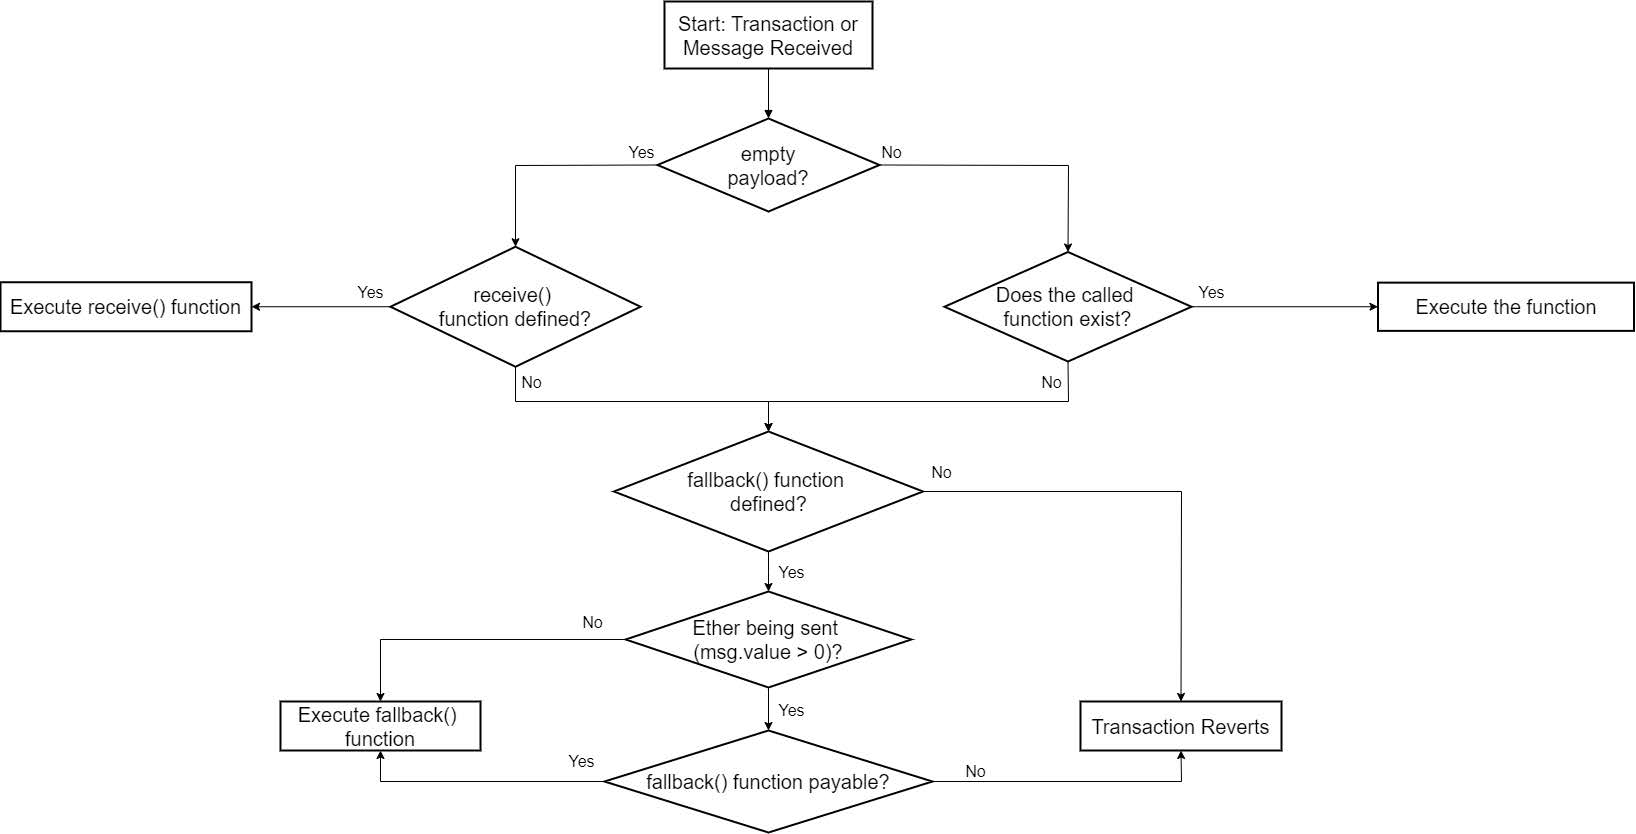
\includegraphics[width=\linewidth]{Images/Receive_and_fallback_functions.jpg}
    \caption{Contract transactions and messages handling}
    \label{fig:transaction_and_message_handling}
\end{figure}

\newpage

\section{The Strict Gas Limitation}

Both the \texttt{receive} function and a \texttt{fallback} function triggered by a simple Ether transfer are subject to a strict gas stipend of \textbf{2,300 gas}. This limit exists because the sending contract sends 2,300 gas to the receiving contract when the former uses the \texttt{transfer} and the \texttt{send} functions (we will cover them later in section ~\ref{sct:methods_for_sending_ether}) and if the receiving contract uses a lesser amount of gas, the remaining part is returned to the sending contract. Minimal balance update functions are much cheaper than 2,300 gas but this small amount exists as a security measure to prevent re-entrancy attacks. Due to this limit, the following operations are forbidden within these functions:

\begin{itemize}
    \item Writing to storage
    \item Creating a new contract
    \item Calling an external function that consumes a large amount of gas
    \item Sending Ether
\end{itemize}

\section{Methods for Sending Ether}
\label{sct:methods_for_sending_ether}

There are three primary methods for a contract to send Ether to another address. They differ significantly in how they forward gas and handle failures (see table ~\ref{lbl:ether_sending_methods}).\\

\begin{table}[h!]
    \centering
    \begin{tabular}{|p{0.25\textwidth}|p{0.25\textwidth}|p{0.5\textwidth}|}
        \hline
        Method & Gas Forwarded & Failure Handling \\ \hline
        
        \texttt{\textbf{transfer(amount)}} & 2,300 gas & Reverts the transaction on failure. \\ \hline
        
        \texttt{\textbf{send(amount)}} & 2,300 gas & Returns \texttt{false} on failure. Does not automatically revert the transaction. \\ \hline
        
        \texttt{\textbf{call\{value: amount[, gas: gasAmount]\}("")}} & Forwards all remaining gas by default (configurable). & Returns \texttt{false} on failure. Recommended for its flexibility and control. It forwards all available gas by default, which can be configured, and allows for calling specific functions on the recipient contract. \\ \hline
    \end{tabular}
    \caption{Ether sending methods}
    \label{lbl:ether_sending_methods}
\end{table}

While \texttt{call} is the recommended method for its control and ability to interact with more complex recipient contracts, its flexibility also introduces the risk of a re-entrancy attack.

\section{The Re-Entrancy Attack Deconstructed}

A re-entrancy attack occurs when a malicious contract exploits a flaw in a victim contract's logic to recursively call a function and drain its funds before its internal state is properly updated. The \texttt{call} method is a key enabler of this attack because it forwards enough gas for the recipient to execute its own complex logic.\\

Let's analyze the vulnerability in a \texttt{VulnerableBank} contract:

\begin{lstlisting}[caption={Vulnerable bank}]
    // Simplified example of a vulnerable contract
    contract VulnerableBank {
        mapping(address => uint) public balances;
    
        function withdraw(uint amount) public {
            // 1. Check if the user has sufficient balance
            require(balances[msg.sender] >= amount);
    
            // 2. Send the Ether *before* updating the balance (THE FLAW)
            (bool success, ) = msg.sender.call{value: amount}("");
            require(success, "Transfer failed.");
    
            // 3. Update the balance *after* the external call
            balances[msg.sender] -= amount;
        }
        // ... other functions
    }
\end{lstlisting}

The flawed logic is the order of operations: it sends Ether \textit{before} it deducts the amount from the user's balance.

\newpage

An \texttt{Attacker} contract can exploit this as follows:

\begin{lstlisting}[caption={Attacker exploit}]
    // Simplified example of an attacker contract
    contract Attacker {
        VulnerableBank public bank;
    
        // ... constructor to set the bank address
    
        function attack() public payable {
            bank.deposit{value: 1 ether}();
            bank.withdraw(1 ether);
        }
    
        // This function is called when the Attacker contract receives Ether
        receive() external payable {
            // As long as the bank has funds, re-enter the withdraw function
            if (address(bank).balance >= 1 ether) {
                bank.withdraw(1 ether);
            }
        }
    }
\end{lstlisting}

The attack unfolds in these steps:

\begin{enumerate}
    \item The attacker calls their \texttt{attack} function, which first deposits 1 Ether into \texttt{VulnerableBank} and then calls \texttt{withdraw(1 ether)}.
    
    \item \texttt{VulnerableBank} checks the attacker's balance (which is 1 Ether) and proceeds. It then uses \texttt{call} to send 1 Ether back to the \texttt{Attacker} contract.
    
    \item The transfer of Ether triggers the \texttt{Attacker} contract's \texttt{receive} function.
    
    \item Crucially, inside its \texttt{receive} function, the \texttt{Attacker} contract immediately calls \\ \texttt{VulnerableBank.withdraw(1 ether)} \textit{again}. This is possible because when the bank uses the \texttt{call} function, it sends enough gas to the attacker for it to perform more complex operations.
    
    \item This recursive call works because the \texttt{VulnerableBank}'s state has not yet been updated. The attacker's balance is still recorded as 1 Ether, so the \texttt{require} check at the very beginning of the \texttt{withdraw} function passes again and again. This loop continues, draining the \texttt{VulnerableBank} of its funds, until the bank's balance is depleted.\\
    To better understand this phenomenon we need to consider that the \texttt{call} function used by the bank waits for the \texttt{receive} function of the attacker to end and return a value containing the outcome of the operation (\texttt{true} for success or \texttt{false} for failure). If the attacker calls the \texttt{withdraw} function again before the \texttt{receive} function ends, it leaves the \texttt{receive} function pending and creates a new \texttt{receive} function. This creates a stack of \texttt{receive} functions until the bank's balance is depleted. This process is similar to a recursive function in which the base case is the one in which the bank has 0 ether and the intermediate case is the one in which the bank has at least 1 ether (see figure ~\ref{fig:re-entrancy_attack_stack}).
\end{enumerate}

\begin{figure}
    \centering
    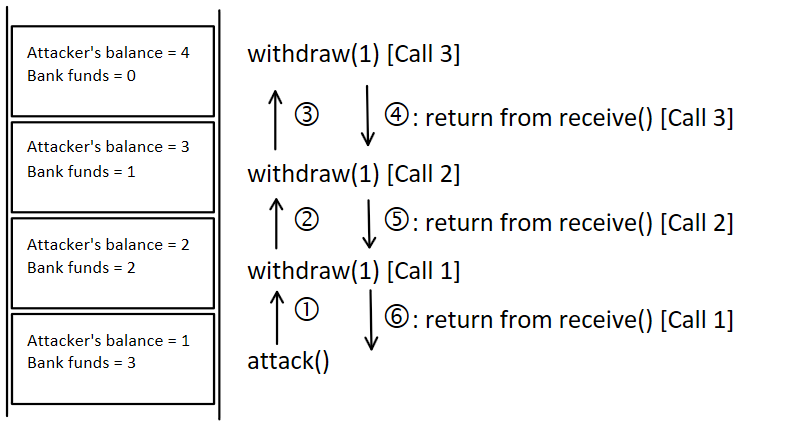
\includegraphics[width=\linewidth]{Images/Re-entrancy attack stack.png}
    \caption{Re-entrancy attack stack - In this example the bank had 2 Ether before the attacker deposited 1 Ether.}
    \label{fig:re-entrancy_attack_stack}
\end{figure}

One might ask: "How does this code deplete all the Ether stored in the bank? Why doesn't it deplete only the balance of the account of the sender?" The answer lies in understanding how the contract manages its funds. The VulnerableBank maintains individual balance records for each user through the balances mapping, but the actual Ether is stored in the contract's own balance. When the bank executes call{value: amount}, it sends Ether from its own balance, not from a segregated account. The balances mapping is merely an internal accounting system that tracks how much each user is allowed to withdraw. Because the contract fails to update this accounting system before sending funds, the attacker can repeatedly pass the require check and drain the contract's entire Ether balance, even though their recorded balance should have been depleted after the first withdrawal. \\

Understanding the nuances of Ether handling is non-negotiable for contract security. After establishing how a contract manages its funds, the next step is to understand how it communicates information about its operations to the outside world.

\chapter{Communicating Off-Chain: Events}

While contracts execute their logic on the blockchain, they often need to communicate information about their state changes to external applications, such as user interfaces or backend services. Solidity \textbf{events} are a crucial and gas-efficient mechanism for this purpose, providing an abstraction over the EVM's logging functionality that allows off-chain applications to subscribe and react to on-chain activity.

\section{Properties and Purpose of Events}

When a contract emits an event, it generates a log record with several key properties:

\begin{itemize}
    \item \textbf{Storage}: Logs are stored in a special data structure within a transaction's receipt, making them a permanent part of the blockchain history.
    
    \item \textbf{Association}: Each log is permanently associated with the address of the contract that emitted it.
    
    \item \textbf{Inheritance}: Events are inheritable members of contracts, just like state variables and functions.
    
    \item \textbf{Inaccessibility}: Critically, logs are \textbf{not accessible from within smart contracts}, not even from the contract that created them. Their sole purpose is to provide a one-way communication channel to the off-chain world.
\end{itemize}

\section{A Publish-Subscribe System}

The most effective way to conceptualize events is as a \textbf{publish-subscribe system}. The smart contract acts as a publisher, broadcasting messages about its activities. Off-chain applications, such as a web frontend, act as subscribers, listening for specific messages that are relevant to them.\\

Let's examine the syntax using the \texttt{ClientReceipt} contract as an example.

\begin{lstlisting}[caption={Client receipt}]
    pragma solidity >=0.4.21 <0.7.0;
    
    contract ClientReceipt {
        // 1. "Topic" Declaration
        event Deposit(
            address indexed _from,
            bytes32 indexed _id,
            uint _value
        );
    
        function deposit(bytes32 _id) public payable {
            // 2. "Publishing" an Event
            emit Deposit(msg.sender, _id, msg.value);
        }
    }
\end{lstlisting}

\begin{enumerate}
    \item \textbf{Declaration and Topics}: The \texttt{event} keyword declares a new message type. Parameters marked with the \texttt{indexed} attribute become \textbf{topics}. These topics create a searchable index that allows subscribers to efficiently filter for specific events (e.g., "show me all \texttt{Deposit} events where the \texttt{\_from} address is \texttt{0x123...}"). Parameters not marked with the \texttt{indexed} attribute are encoded into the data part of the log.
    
    \item \textbf{Emission (Publishing)}: The \texttt{emit} keyword is used within a function to "publish" an event. This action records the event's arguments in the transaction's log, making the message available for any subscribed off-chain application to consume.
\end{enumerate}

Events serve as a vital, one-way communication channel from the on-chain world of smart contracts to the off-chain world of user applications. To create robust systems, contracts also need standardized ways to interact with each other, which is achieved by defining contract blueprints.

\chapter{Defining Blueprints: Interfaces}

Solidity \textbf{interfaces} provide a way to define a contract's external-facing functions without implementing them. They serve a purpose similar to abstract contracts but are more restrictive, acting as a pure blueprint or Application Binary Interface (ABI) that other contracts can be expected to adhere to. This allows for contract-to-contract interaction without needing the full source code of the target contract, only its interface.

\section{Interface Restrictions}

Interfaces are defined by the \texttt{interface} keyword and must follow a strict set of rules that distinguish them from abstract contracts:

\begin{itemize}
    \item They cannot have any functions with implementations.
    \item They cannot inherit from other contracts or interfaces.
    \item All declared functions must be marked as \texttt{external}.
    \item They cannot declare a constructor.
    \item They cannot declare state variables.
\end{itemize}

Ultimately, interfaces, combined with strategic function visibility and a well-designed inheritance hierarchy, provide developers with a complete toolkit for building complex, modular, and secure systems where disparate components can interact with predictable and guaranteed behavior.

\chapter{Understanding Solidity Libraries for Reusable and Secure Code}

Solidity libraries are a powerful mechanism for promoting code reuse within the Ethereum ecosystem. Their strategic importance lies in creating modular, gas-efficient, and secure smart contracts by isolating common logic into a single, verifiable module. A library is deployed only once to a specific blockchain address, and its code can then be referenced and executed by multiple contracts, saving deployment costs and centralizing functionality.\\

The core characteristics of a Solidity library distinguish it from a standard contract:

\begin{itemize}
    \item \textbf{Single Deployment \& Code Reuse:} Libraries are designed to be deployed once to a permanent address, allowing any number of other contracts to link to and reuse their functions.
    
    \item \textbf{Stateless Nature:} Libraries are fundamentally stateless. They do not have their own state variables and cannot hold a balance. Instead, they operate on the state variables of the contract that calls them, provided those variables are explicitly passed as arguments.
    
    \item \textbf{Caller's Context Execution:} When a contract calls a library function, the function's code is executed within the context of the \textit{calling contract}. This means that the \texttt{this} keyword inside the library function refers to the calling contract, and the library code can directly access and modify the caller's storage.
\end{itemize}

This unique execution context is enabled by the Ethereum Virtual Machine's (EVM) \\
\texttt{delegatecall} instruction, which stands in contrast to the standard \texttt{call} instruction. A \texttt{call} creates a new execution context where \texttt{this} refers to the called contract and the code operates on its own storage. Conversely, \texttt{delegatecall} is the mechanism that allows a library's code to function as if it were an internal part of the caller, preserving the calling contract's context and operating directly on its state.\\

To illustrate this, consider a contract \texttt{C} that uses a \texttt{Set} library to manage a data structure. First, the contract \texttt{C} is defined:

\begin{lstlisting}[caption={Contract that uses a 'Set' library}, label={lst:library_user}]
    contract C {
        Data knownValues;
    
        function register(uint value) public {
            // Library functions are called directly on the library name
            // without creating an instance.
            Set.insert(knownValues, value);
        }
    }
\end{lstlisting}

The data structure and the library logic used by contract \texttt{C} are defined as follows:

\begin{lstlisting}[caption={Data structure and library logic used by contract C}, label={lst:library_code}]
    struct Data {
        mapping(uint => bool) flags;
    }
    
    library Set {
        // The first parameter is a storage reference to the calling
        // contract's state variable. 'self' is the idiomatic name.
        function insert(Data storage self, uint value)
        public returns (bool) {
            if (self.flags[value])
                return false; // already there
            self.flags[value] = true;
            return true;
        }
    
        function remove(Data storage self, uint value)
        public returns (bool) {
            if (!self.flags[value])
                return false; // not there
            self.flags[value] = false;
            return true;
        }
    
        function contains(Data storage self, uint value)
        public view returns (bool) {
            return self.flags[value];
        }
    }
\end{lstlisting}

This implementation highlights several key features. Notice that the library function is called directly on the library name (\texttt{Set.insert(...)}) without creating an instance, unlike standard contracts which require instantiation before use. The \texttt{insert} function's first parameter, \texttt{self}, is of the type \texttt{Data storage reference}. This allows the calling contract's \texttt{knownValues} state variable to be passed by its address rather than its content. This is a critical performance optimization, as it avoids the costly and gas-intensive process of copying the entire \texttt{Data} struct into memory. By using this reference, the library function can directly and efficiently modify the calling contract's storage. The use of \texttt{self} as the parameter name is an idiomatic convention, reinforcing the idea that the function is acting as a method on the data object it receives.\\

Actually, the code in the slides is a simplified version of its real-world counterpart. In fact, you can notice that there isn't an explicit library declaration in code ~\ref{lst:library_code} and there isn't an explicit library importation in code ~\ref{lst:library_user}. The real-world code is the following:

\begin{lstlisting}[caption={Real world library declaration and usage}]
    pragma solidity >=0.6.0 <0.9.0;

    library Set { // EXPLICIT LIBRARY DECLARATION
        struct Data {
            mapping(uint => bool) flags;
        }
        
        function insert(Data storage self, uint value) internal returns (bool) {
            if (self.flags[value])
                return false;
            self.flags[value] = true;
            return true;
        }
        // ... other functions
    }
    
    contract C {
        // EXPLICIT LIBRARY IMPORTATION AND ASSOCIATION TO A DATA TYPE
        using Set for Data;
        Data knownValues;
        
        function register(uint value) public {
            knownValues.insert(value);
        }
    }
\end{lstlisting}

It's important to notice that libraries are associated to a specific data type when imported meaning that the library under discussion can be used to handle its associated data type. It is also possible to import the same library multiple times to associate it to different data types as follows:

\begin{lstlisting}[caption={Importing the same library multiple times to associate it to different data types}]
    using Set for Data1; using Set for Data2;
\end{lstlisting}

While libraries provide reusable logic, that logic must often react to the state of the blockchain itself. To do this, Solidity provides a rich set of global variables and functions that expose the execution context.

\chapter{Accessing Blockchain State with Global Variables and Functions}

Solidity provides a set of special, globally-available variables and functions that can be accessed from within any smart contract. Their strategic importance is immense, as they enable contracts to access critical information about the blockchain, the current transaction, and the specific message call. This context-awareness is essential for implementing core logic, such as access control, timestamp-based operations, and payment verification. It's important to note that this set of variables evolves with the Ethereum protocol; for instance, \texttt{block.difficulty} was deprecated following Ethereum's transition to a Proof-of-Stake consensus mechanism.\\

The key global variables and functions are grouped below by the context they describe.

\section{Block Properties}

\begin{table}[h!]
    \centering
    \begin{tabular}{|p{0.3\textwidth}|p{0.2\textwidth}|p{0.4\textwidth}|}
        \hline
        Variable/Function & Type & Description \\ \hline
        \texttt{block.number} & \texttt{uint} & The current block number. \\ \hline
        \texttt{block.timestamp} & \texttt{uint} & The current block timestamp as seconds since the UNIX epoch. \\ \hline
        \texttt{block.coinbase} & \texttt{address} & The address of the current block's miner. \\ \hline
        \texttt{block.gaslimit} & \texttt{uint} & The gas limit for the current block. \\ \hline
    \end{tabular}
\end{table}

\section{Transaction Properties}

\begin{table}[h!]
    \centering
    \begin{tabular}{|p{0.3\textwidth}|p{0.2\textwidth}|p{0.4\textwidth}|}
        \hline
        Variable/Function & Type & Description \\ \hline
        \texttt{tx.origin} & \texttt{address} & The original sender of the transaction (the full call chain). \\ \hline
        \texttt{tx.gasprice} & \texttt{uint} & The gas price of the transaction. \\ \hline
    \end{tabular}
\end{table}

\newpage

\section{Message Properties}

\begin{table}[h!]
    \centering
    \begin{tabular}{|p{0.3\textwidth}|p{0.2\textwidth}|p{0.4\textwidth}|}
        \hline
        Variable/Function & Type & Description \\ \hline
        \texttt{msg.sender} & \texttt{address} & The sender of the immediate message (the current call). \\ \hline
        \texttt{msg.value} & \texttt{uint} & The number of wei sent with the message. \\ \hline
        \texttt{msg.data} & \texttt{bytes} & The complete calldata. \\ \hline
        \texttt{msg.sig} & \texttt{bytes4} & The first four bytes of the calldata (the function identifier). \\ \hline
    \end{tabular}
\end{table}

\section{Gas Management}

\begin{table}[h!]
    \centering
    \begin{tabular}{|p{0.3\textwidth}|p{0.2\textwidth}|p{0.4\textwidth}|}
        \hline
        Variable/Function & Type & Description \\ \hline
        \texttt{gasleft()} & \texttt{uint256} & The amount of remaining gas for the current execution. \\ \hline
    \end{tabular}
\end{table}

A critical distinction to understand is between \texttt{msg.sender} and \texttt{tx.origin}. While both refer to an address, \texttt{msg.sender} identifies the immediate caller of the current function, which could be an Externally Owned Account (EOA) or another smart contract. In contrast, \texttt{tx.origin} always refers to the original EOA that initiated the entire transaction chain. If an EOA calls Contract A, which in turn calls Contract B, then within Contract B, \texttt{msg.sender} will be the address of Contract A, while \texttt{tx.origin} will be the address of the initial EOA. For this reason, using \texttt{tx.origin} for authorization is a significant security risk, as it can make a contract vulnerable to phishing attacks. Best practice dictates using \texttt{msg.sender} for access control logic.\\

These global variables provide a snapshot of the blockchain's state during a transaction, but to understand the full picture, we must first examine the transaction that places the contract on the chain to begin with: deployment.

\chapter{The Smart Contract Lifecycle: Deployment and Bytecode Structure}

Deploying a smart contract is the process that establishes its permanent presence and code on the Ethereum blockchain. This is not an abstract event but a standard transaction with a specific payload. A contract is deployed by sending a transaction that has no \texttt{to} address specified; instead, the transaction's \texttt{data} field contains the contract's creation bytecode, which includes both the initialization code and any ABI-encoded arguments required by the contract's constructor.\\

The deployment bytecode sent in this transaction consists of three primary components (see the right part of figure ~\ref{fig:smart_contract_deployment}):

\begin{enumerate}
    \item \textbf{Constructor Code:} This is the initialization code that runs only once during the contract's deployment. Its purpose is twofold: first, to execute the logic defined in the contract's \texttt{constructor} function, and second, to return the runtime bytecode of the contract.
    
    \item \textbf{Runtime Bytecode:} This is the actual logic of the smart contract that is permanently stored on the blockchain at the newly created contract's address. This code is executed every time a function is called on the contract after deployment.
    
    \item \textbf{Metadata:} Additional metadata is also appended to the bytecode, providing supplementary information about the contract.
\end{enumerate}

\begin{figure}
    \centering
    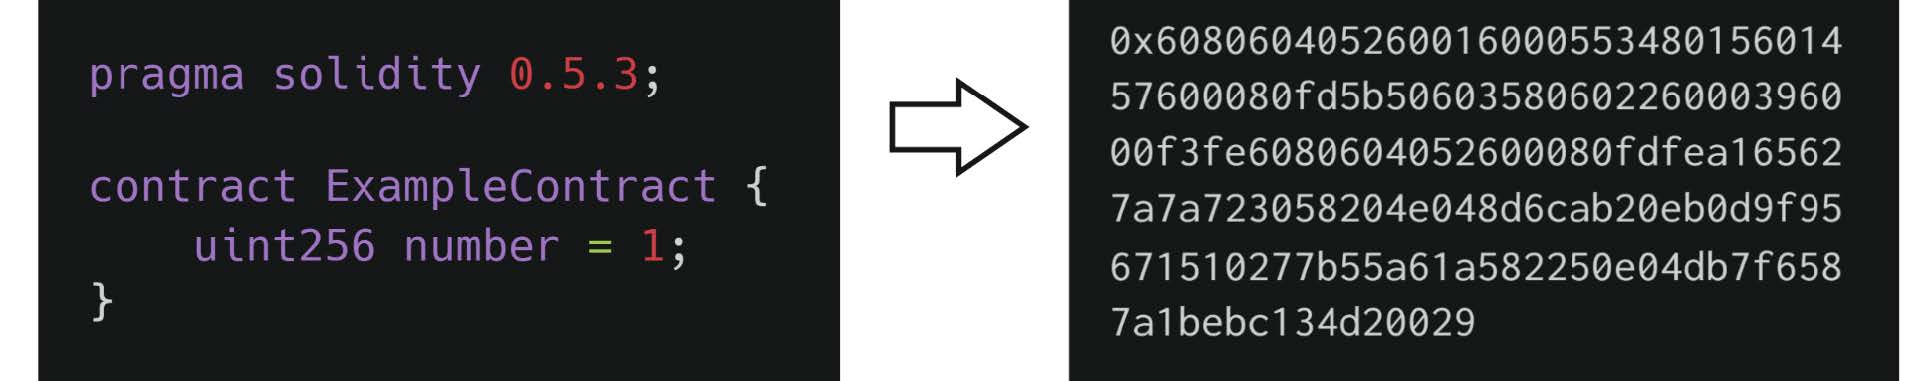
\includegraphics[width=\linewidth]{Images/Deploying_a_smart_contract.jpg}
    \caption{Deploying a smart contract}
    \label{fig:smart_contract_deployment}
\end{figure}

Once this bytecode is created and stored on-chain, external applications and other contracts require a standardized interface to communicate with it.

\chapter{The Application Binary Interface (ABI): The Language of Smart Contracts}

\begin{figure}
    \centering
    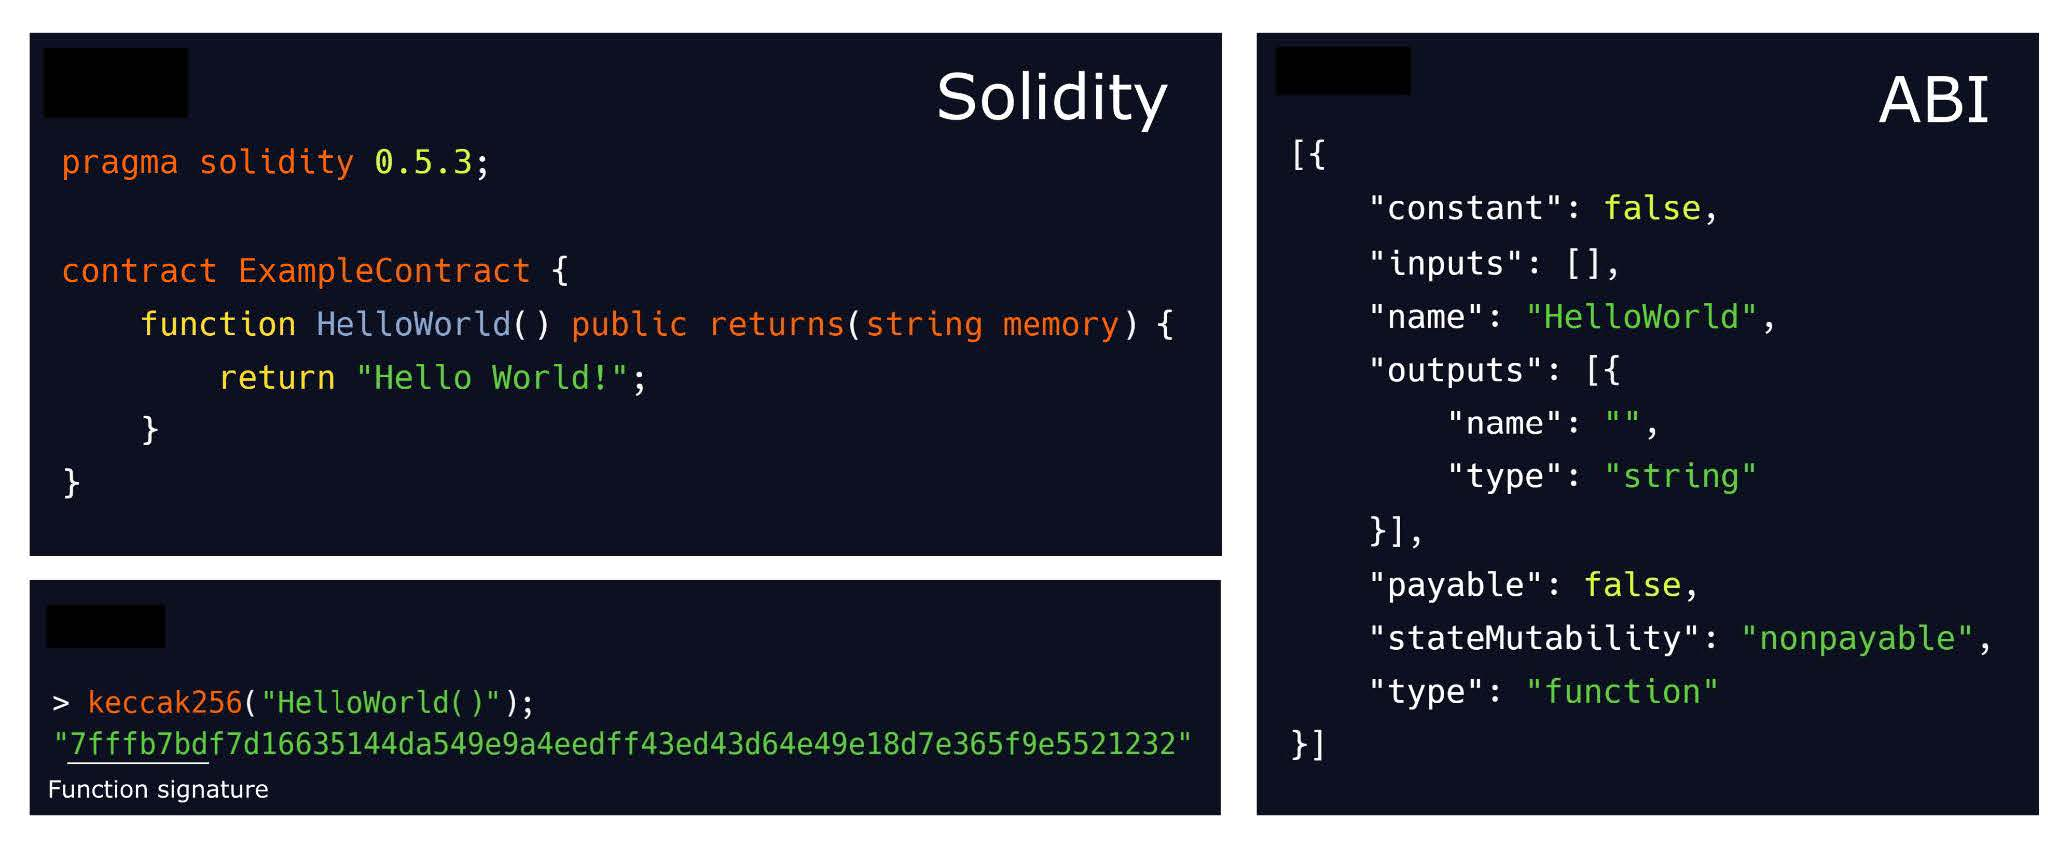
\includegraphics[width=\linewidth]{Images/Contract_ABI_example.jpg}
    \caption{Contract ABI example}
    \label{fig:contract_abi_example}
\end{figure}

The Contract Application Binary Interface (ABI) is the standard for interacting with functions in an Ethereum smart contract, defining the rules for encoding and decoding data sent to and from the EVM. Its strategic importance cannot be overstated, as it provides the "user manual" for a contract's bytecode, defining precisely how to call its functions and receive data back. The ABI is essential for communication, whether from an external application (like DApps, Decentralized applications which are open-source software programs that run on peer-to-peer blockchain networks rather than centralized servers) or from another contract on the blockchain.\\

An ABI-encoded function call has a well-defined structure that is placed in the \texttt{calldata} of a transaction or message:

\begin{itemize}
    \item \textbf{Function Selector:} The first four bytes of the \texttt{calldata} uniquely identify the function being called. This selector is generated by taking the first four bytes of the Keccak-256 hash of the function's signature (on the bottom left part of figure ~\ref{fig:contract_abi_example}). The signature is a string composed of the function's name and its argument types, with no spaces and without variable names (e.g., \texttt{register(string)}).
    
    \item \textbf{Encoded Arguments:} Following the four-byte function selector, starting from the fifth byte, are the function's arguments. Each argument is encoded into 32-byte words according to the strict rules laid out in the official ABI specification.
\end{itemize}

It is important to differentiate between the ABI specification itself and the ABI JSON file. The ABI is the formal set of encoding and decoding rules. When you compile a Solidity contract, the compiler also generates a separate ABI JSON file (see the right part of figure ~\ref{fig:contract_abi_example}). This file is a detailed, machine-readable description of the contract's public interface, including all of its public and external functions, their parameters, events, and errors. Tools, libraries, and DApps use this JSON file to automatically handle the encoding and decoding process, abstracting the low-level complexity away from developers.\\

While high-level contract interactions in Solidity often handle ABI encoding automatically, it is also possible to construct a low-level call manually. The following example demonstrates using a low-level \texttt{call} where the calldata must be explicitly encoded according to the ABI:

\begin{lstlisting}
    address(nameReg).call{gas: 1000000, value: 1 ether}(
        abi.encodeWithSignature("register(string)", "MyName")
    );
\end{lstlisting}

In this code, rather than calling a function on a contract instance directly, a generic \texttt{call} is made to the \texttt{nameReg} address. The developer must manually provide the ABI-encoded \texttt{calldata}. The \texttt{abi.encodeWithSignature} function is a built-in Solidity utility that generates the required bytes by creating the function selector from the signature \texttt{"register(string)"} and encoding the string argument \texttt{"MyName"}.\\

Mastery of these concepts—from writing modular logic with libraries, to querying the chain state with global variables, and defining a clear communication protocol with the ABI—is what separates a functional smart contract from a secure, efficient, and interoperable decentralized application.

\end{document}
